\chapter{Arhitektura i dizajn sustava}

		Arhitektura koju koristimo se zasniva na MVC (Model-View-Controller) konceptu, varijacije arhitekture zasnovane na događajima.
        \\
        \\
        Cjelokupni sustav se može podijeliti na četiri glavne komponente:
            \begin{itemize}
                \item Web preglednik
                \item Web poslužitelj (server)
                \item Web aplikaciju
                \item Bazu podataka
            \end{itemize}
    
        \begin{figure}[h]
            \centering
            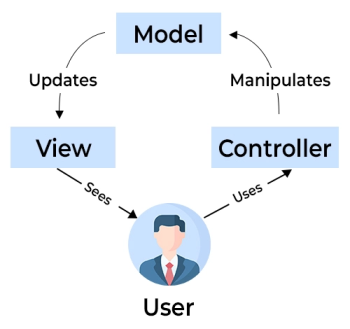
\includegraphics[width=0.5\textwidth]{slike/mvc.png}
            \caption{MVC model}
            \label{fig:mesh1}
        \end{figure}
        
        \textbf{Web preglednik} je program (software) koji omogućava korisnicima pregledavanje i prikazivanje web stranica na World Wide Webu (WWW). Predstavlja sučelje između korisnika i internetskog sadržaja. Pomoću njega korisnik sustava komunicira s web aplikacijom, točnije \textit{View} i \textit{Controller} komponentom.
        
        \pagebreak

        \textbf{Web aplikaciju} pokreće \textbf{poslužitelj}. To je program čiji je osnovni zadatak odgovarati na HTTP (\textit{Hyper Text Transfer Protocol}) zahtjeve klijenata, primati i slati određene resurse - posluživati samu aplikaciju. 
        
        \begingroup 
        U većini slučajeva klijent će zahtjevati pristup podacima kojima web poslužitelj nema pristup. U tom slučaju će \textit{Controller} komponenta poslati zahtjev \textit{Model} komponenti, zaslužnoj za pohranu korisničkih podataka, koju u našem slučaju predstavlja \textbf{baza podataka}. 
        \endgroup
        
        \begingroup
        Baza podataka organizirana je zbirka logički povezanih, pretražljivih i međusobno ovisnih podataka. Ključna je komponenta mnogih aplikacija i sustava zbog mogućnosti sigurne pohrane i brzog pretraživanja SQL upitima.
	  \endgroup

        \begingroup
        Za našu implementaciju korisničkog sučelja odabrali smo programski jezik \textit{JavaScript} s bibliotekom \textit{React}. Za implementaciju poslužiteljske strane odabrali smo programski jezik \textit{Java} i \textit{Spring} framework, točnije proširenje \textit{Spring Boot}. Kao razvojnu okolinu odabrali smo \textit{Visual Studio Code} i \textit{JetBrains IntelliJ IDEA}. Za implementaciju baze podataka odabrali smo \textit{PostgreSQL}.
        \endgroup

		\begin{figure}[h]
            \centering
            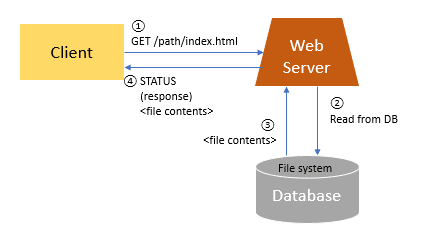
\includegraphics[width=1\textwidth]{slike/client-server-db.png}
            \caption{Prikaz osnovnog rada sustava}
            \label{fig:mesh1}
        \end{figure}

        \pagebreak
				
		\section{Baza podataka}
			
		\noindent Za naš sustav koristit ćemo relacijsku bazu podataka, koja je strukturno pogodna za modeliranje stvarnog svijeta. Osnovna komponenta ove baze je relacija, koja se definira svojim imenom i skupom atributa. Glavna svrha ove baze podataka je omogućiti brzo i jednostavno pohranjivanje, mijenjanje i dohvaćanje podataka radi daljnje obrade. Baza podataka za ovu aplikaciju uključuje sljedeće entitete:
		
		\begin{packed_item}
			
			\item Korisnik
			\item Registrirani			
			\item Skloniste
			\item Oglas
			\item Ljubimac
			\item Lokacija
			\item Mjesto
			\item Zupanija
			\item Slika
			\item Poruka
			\item Kategorija
			
		\end{packed_item}
		
			\subsection{Opis tablica}
			

				\noindent \textbf{Korisnik} Entitet sadržava sve važne informacije o korisniku web-aplikacije. Atributi su sljedeći: sifKorisnik, korisnickoIme, lozinka, email, telefon, postBr. Primarni ključ ovog entiteta je atribut sifKorisnik. Entitet je povezan s entitetom Mjesto pomoću atributa postBr kroz vezu \textit{Many-to-One}, a s entitetima Registrirani i Skloniste, kao specijalizacije, pomoću atributa korisnickoIme. Postoji i povezanost vezom \textit{One-to-Many} s identifikacijskim slabim entitetom Poruka pomoću atributa korisnickoIme.
				
				
				\begin{longtblr}[
					label=none,
					entry=none
					]{
						width = \textwidth,
						colspec={|X[6,l]|X[6, l]|X[20, l]|}, 
						rowhead = 1,
					} %definicija širine tablice, širine stupaca, poravnanje i broja redaka naslova tablice
					\hline \SetCell[c=3]{c}{\textbf{Korisnik }}	 \\ \hline[3pt]
					\SetCell{LightGreen}sifKorisnik & VARCHAR	&  	jedinstvena šifra korisnika  	\\ \hline korisnickoIme & VARCHAR	&  	korisničko ime  	\\ \hline
					lozinka	& VARCHAR & hash lozinke  	\\ \hline 
					email & VARCHAR & e-mail adresa korisnika  \\ \hline 
					telefon & VARCHAR	& telefonski broj korisnika 		\\ \hline 
					\SetCell{LightBlue} postBr	& INT & poštanski broj mjesta stanovanja korisnika  	\\ \hline 
				\end{longtblr}
				
				
				\noindent \textbf{Registrirani} Entitet je specijalizacija entiteta Korisnik i sadrži dodatne podatke o registriranom korisniku. Atributi entiteta su ime, prezime i korisnickoIme. Entitet je kao specijalizacija povezan entitetom Korisnik kroz atribut korisnickoIme.
				
				
				\begin{longtblr}[
					label=none,
					entry=none
					]{
						width = \textwidth,
						colspec={|X[6,l]|X[6, l]|X[20, l]|}, 
						rowhead = 1,
					} %definicija širine tablice, širine stupaca, poravnanje i broja redaka naslova tablice
					\hline \SetCell[c=3]{c}{\textbf{Registrirani }}	 \\ \hline[3pt]
					ime	& VARCHAR & ime registriranog korisnika  	\\ \hline 
					prezime & VARCHAR & prezime registriranog korisnika  \\ \hline 
					\SetCell{LightBlue} korisnickoIme	& VARCHAR & jedinstveno korisničko ime	\\ \hline 
				\end{longtblr}
				
				
				\noindent \textbf{Skloniste} Entitet je specijalizacija entiteta Korisnik i sadrži dodatne podatke o skloništu za životinje. Atributi entiteta su nazivSklonista i korisnickoIme. Entitet je kao specijalizacija povezan entitetom Korisnik kroz atribut korisnickoIme.
				
				
				\begin{longtblr}[
					label=none,
					entry=none
					]{
						width = \textwidth,
						colspec={|X[6,l]|X[6, l]|X[20, l]|}, 
						rowhead = 1,
					} %definicija širine tablice, širine stupaca, poravnanje i broja redaka naslova tablice
					\hline \SetCell[c=3]{c}{\textbf{Skloniste }}	 \\ \hline[3pt]
					nazivSklonista & VARCHAR	&  	naziv skloništa za životinje  	\\ \hline
					\SetCell{LightBlue}korisnickoIme	& VARCHAR & jedinstveno korisničko ime  	\\ \hline
				\end{longtblr}
				
				
				\noindent \textbf{Ljubimac} Entitet sadržava sve važne podatke o kućnome ljubimcu. Atributi entiteta su: sifLjubimac, ime, vrsta, starost, boja, opis. Primarni ključ ovog entiteta je atribut sifLjubimac. 
				Entitet je povezan vezom \textit{One-to-Many} kroz atribut sifLjubimac s entitetom Slika. Također, postoji veza \textit{One-to-Many} s entitetom Oglas pomoću atributa sifOglas.
				
				\begin{longtblr}[
					label=none,
					entry=none
					]{
						width = \textwidth,
						colspec={|X[6,l]|X[6, l]|X[20, l]|}, 
						rowhead = 1,
					} %definicija širine tablice, širine stupaca, poravnanje i broja redaka naslova tablice
					\hline \SetCell[c=3]{c}{\textbf{Ljubimac }}	 \\ \hline[3pt]
					\SetCell{LightGreen}sifLjubimac & INT	&  	jedinstvena šifra ljubimca  	\\ \hline
					ime	& VARCHAR & ime na koje se ljubimac odaziva  	\\ \hline 
					vrsta & VARCHAR & vrsta ljubimca  \\ \hline 
					starost & INT	& starost ljubimca 		\\ \hline 
					boja & VARCHAR & boja ljubimca  \\ \hline 
					opis & VARCHAR	& dodatan opis ljubimca 		\\ \hline 
				\end{longtblr}
				
				
				\noindent \textbf{Oglas} Entitet sadržava sve važne informacije o oglasu za kućnog ljubimca. Atributi su sljedeći: sifOglas, datumVrijemeNestanka, koordinate, sifLjubimac, sifKategorija, korisnickoIme. Primarni ključ ovog entiteta je atribut sifOglas. Entitet je u vezi \textit{Many-to-One} s entitetom Lokacija pomoću atributa koordinate, u vezi \textit{Many-to-One} s entitetom Ljubimac pomoću atributa sifLjubimac, u vezi \textit{Many-to-One} s entitetom Kategorija pomoću atributa sifKategorija te u vezi \textit{Many-to-One} s entitetom Korisnik pomoću atributa korisnickoIme.
				
				
				\begin{longtblr}[
					label=none,
					entry=none
					]{
						width = \textwidth,
						colspec={|X[10,l]|X[6, l]|X[16, l]|}, 
						rowhead = 1,
					} %definicija širine tablice, širine stupaca, poravnanje i broja redaka naslova tablice
					\hline \SetCell[c=3]{c}{\textbf{Oglas }}	 \\ \hline[3pt]
					\SetCell{LightGreen}sifOglas & INT	&  	jedinstveni identifikator oglas  	\\ \hline
					datumVrijemeNestanka	& TIMESTAMP & datum i vrijeme nestanka ljubimca  	\\ \hline 
					\SetCell{LightBlue}koordinate & VARCHAR & koordinate lokacije nestanka ljubimca  \\ \hline 
					\SetCell{LightBlue}sifLjubimac & INT	& jedinstveni identifikator ljubimca 		\\ \hline 
					\SetCell{LightBlue} sifKategorija	& INT & jedinstveni identifikator kategorije oglasa  	\\ \hline
					\SetCell{LightBlue}korisnickoIme & VARCHAR & jedinstveno korisničko ime korisnika koji je postavio oglas \\ \hline
					 
				\end{longtblr}
				
				
				\noindent \textbf{Lokacija} Entitet sadržava podatke o lokaciji. Atributi entiteta su sifLokacija, geografskaSirina, geografskaDuzina, imeLokacije i postBr, gdje je primarni ključ atribut sifLokacija. Postoji veza \textit{Many-to-One} s entitetom Mjesto kroz atribut postBr.
				
				
				\begin{longtblr}[
					label=none,
					entry=none
					]{
						width = \textwidth,
						colspec={|X[8,l]|X[6, l]|X[18, l]|}, 
						rowhead = 1,
					} %definicija širine tablice, širine stupaca, poravnanje i broja redaka naslova tablice
					\hline \SetCell[c=3]{c}{\textbf{Lokacija }}	 \\ \hline[3pt]
					\SetCell{LightGreen}sifLokacija & VARCHAR	&  	jedinstvena šifra lokacija  	\\ \hline geografskaSirina & VARCHAR	&  	geografska širina  	\\ \hline geografskaDuzina & VARCHAR	&  	geografska dužina  	\\ \hline imeLokacija & VARCHAR	&  	ime lokacije  	\\ \hline koordinate & VARCHAR	&  	jedinstvene koordinate lokacije  	\\ \hline
					\SetCell{LightBlue} postBr	& INT & poštanski broj mjesta	\\ \hline 
				\end{longtblr}
				
				
				\noindent \textbf{Mjesto} Entitet je sastavljen od podataka vezanih za mjesto pomoću atributa postBr, koji je primarni ključ, nazivMjesto i sifZup. Postoje veze \textit{One-to-Many} pomoću atributa postBr s entitetima Lokacija i Korisnik te veza \textit{Many-to-One} s entitetom Zupanija pomoću atributa sifZup.
				
				
				\begin{longtblr}[
					label=none,
					entry=none
					]{
						width = \textwidth,
						colspec={|X[6,l]|X[6, l]|X[20, l]|}, 
						rowhead = 1,
					} %definicija širine tablice, širine stupaca, poravnanje i broja redaka naslova tablice
					\hline \SetCell[c=3]{c}{\textbf{Mjesto }}	 \\ \hline[3pt]
					\SetCell{LightGreen}postBr & INT	&  	poštanski broj mjesta	\\ \hline
					nazivMjesto	& VARCHAR & naziv mjesta  	\\ \hline 
					\SetCell{LightBlue} sifZup	& INT & jedinstveni identifikator županije	\\ \hline 
				\end{longtblr}
				
				
				\noindent \textbf{Zupanija} Entitet je sastavljen od podataka vezanih za županiju pomoću atributa sifZup i nazivZup. Primarni ključ je sifZup. Postoji veza \textit{One-to-Many} pomoću atributa sifZup s entitetom Mjesto.
				
				
				\begin{longtblr}[
					label=none,
					entry=none
					]{
						width = \textwidth,
						colspec={|X[6,l]|X[6, l]|X[20, l]|}, 
						rowhead = 1,
					} %definicija širine tablice, širine stupaca, poravnanje i broja redaka naslova tablice
					\hline \SetCell[c=3]{c}{\textbf{Zupanija }}	 \\ \hline[3pt]
					\SetCell{LightGreen}sifZup & INT	&  	jedinstveni identifikator županije  	\\ \hline
					nazivZup	& VARCHAR & naziv županije  	\\ \hline 
				\end{longtblr}
				
				
				\noindent \textbf{Poruka} Entitet sadržava sve važne informacije o poruci te je oblikovan kao identifikacijski slabi entitet. Atributi su sljedeći: tekstPoruke, datumVrijemeSlanja, korisnickoIme, koordinate, vezaNaSliku i sifOglas.  Entitet je povezan s entitetom Korisnik pomoću atributa korisnickoIme kroz vezu \textit{Many-to-One}, s entitetom Lokacija kroz vezu \textit{Many-to-One} pomoću atributa koordinate te s entitetom Oglas kroz vezu \textit{Many-to-One} pomoću atributa sifOglas.
				
				
				\begin{longtblr}[
					label=none,
					entry=none
					]{
						width = \textwidth,
						colspec={|X[9,l]|X[6, l]|X[17, l]|}, 
						rowhead = 1,
					} %definicija širine tablice, širine stupaca, poravnanje i broja redaka naslova tablice
					\hline \SetCell[c=3]{c}{\textbf{Poruka }}	 \\ \hline[3pt]
					tekstPoruke & VARCHAR & tekst poruke \\ \hline
					\SetCell{LightBlue}datumVrijemeSlanja & TIMESTAMP	&  	datum i vrijeme slanja poruke  	\\ \hline
					\SetCell{LightBlue}korisnickoIme	& VARCHAR & jedinstveno korisnicko ime  	\\ \hline 
					\SetCell{LightBlue}koordinate & VARCHAR & jedinstvene koordinate lokacije  \\ \hline 
					\SetCell{LightBlue}vezaNaSliku & VARCHAR	& jedinstvena poveznica do slike 		\\ \hline 
					\SetCell{LightBlue}sifOglas & INT	& jedinstveni identifikator oglasa 		\\ \hline 
				\end{longtblr}
				
				
				\noindent \textbf{Slika} Entitet sadržava podatke o slici. Atributi su vezaNaSliku, koji je primarni ključ, i sifLjubimac. S entitetom su povezani: Ljubimac s vezom \textit{Many-to-One} pomoću atributa sifLjubimac, Poruka s vezom \textit{One-to-Many} uz pomoć atributa vezaNaSliku.
				
				
				\begin{longtblr}[
					label=none,
					entry=none
					]{
						width = \textwidth,
						colspec={|X[6,l]|X[6, l]|X[20, l]|}, 
						rowhead = 1,
					} %definicija širine tablice, širine stupaca, poravnanje i broja redaka naslova tablice
					\hline \SetCell[c=3]{c}{\textbf{Slika }}	 \\ \hline[3pt]
					\SetCell{LightGreen}vezaNaSliku & VARCHAR	&  	jedinstvena poveznica do slike  	\\ \hline
					\SetCell{LightBlue}sifLjubimac	& INT & jedinstveni identifikator ljubimca  	\\ \hline  
				\end{longtblr}
				
				
				\noindent \textbf{Kategorija} Entitet se sastoji od podataka o kategoriji: sifKategorija (primarni ključ) i opisKategorija. Postoji veza \textit{One-to-Many} između entiteta Kategorija i Oglasa kroz atribut sifKategorija.
				
				
				\begin{longtblr}[
					label=none,
					entry=none
					]{
						width = \textwidth,
						colspec={|X[6,l]|X[6, l]|X[20, l]|}, 
						rowhead = 1,
					} %definicija širine tablice, širine stupaca, poravnanje i broja redaka naslova tablice
					\hline \SetCell[c=3]{c}{\textbf{Kategorija }}	 \\ \hline[3pt]
					\SetCell{LightGreen}sifKategorija & INT	&  	jedinstveni identifikator kategorije  	\\ \hline
					opisKategorija	& VARCHAR & opis kategorije  	\\ \hline 
				\end{longtblr}
				
			
			\subsection{Dijagram baze podataka}
				\begin{figure}[h]
					\centering
					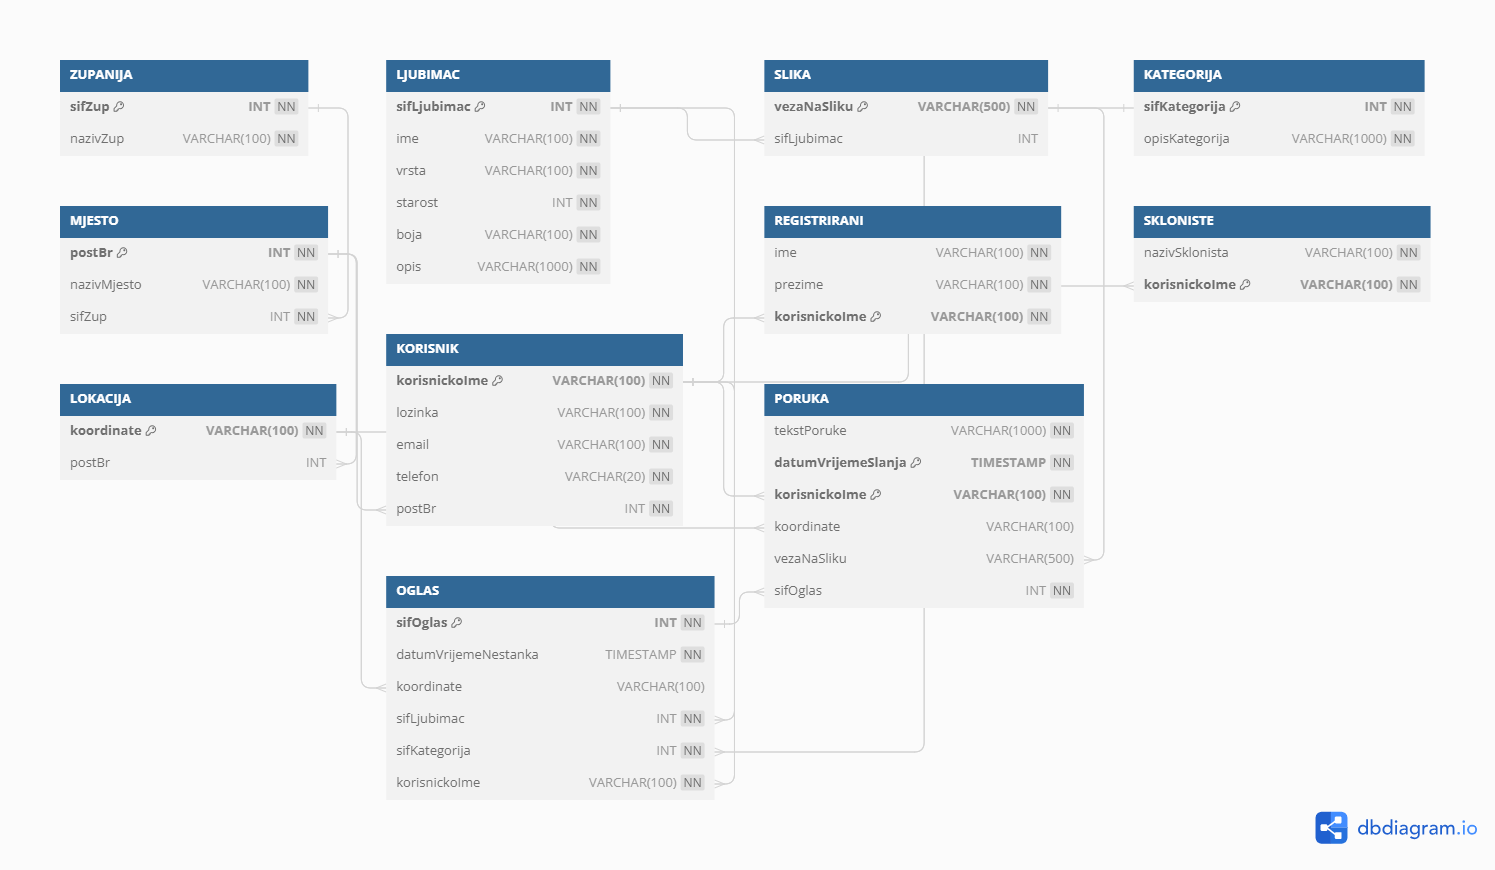
\includegraphics[width=1\textwidth]{slike/ERdiagram.png}
					\caption{E-R dijagram baze podataka}
					\label{fig:mesh1}
				\end{figure}
			
			\eject
			
			
		\section{Dijagram razreda}

                \noindent Na slikama 4.4, 4.5, 4.6 i 4.7 su prikazani razredi koji pripadaju \textit{backend} dijelu MVC arhitekture. Na slici 4.4 je vidljiv paket \textit{controller} koji dijelimo na razrede. Metode koje su implementirane u tim razredima koriste DTO-ove\textit{(Data transfer object)}, a njima pristupamo putem metoda koje su implementirane u \textit{entity} razredima. Metode unutar \textit{controller} paketa vraćaju JSON objekte s odgovarajućim HTTP status kodovima.
			
			Razredi su strukturirani prema pravima pristupa metodama            različitih aktora kako bi se rasteretio dijagram od prevelike       složenosti. Prikazane su samo ovisnosti između razreda unutar       istog segmenta dijagrama. Na osnovu naziva i tipova atributa        unutar razreda, može se zaključiti vrsta veza među različitim       entitetima.

			\begin{figure}[htb]
				\centering
				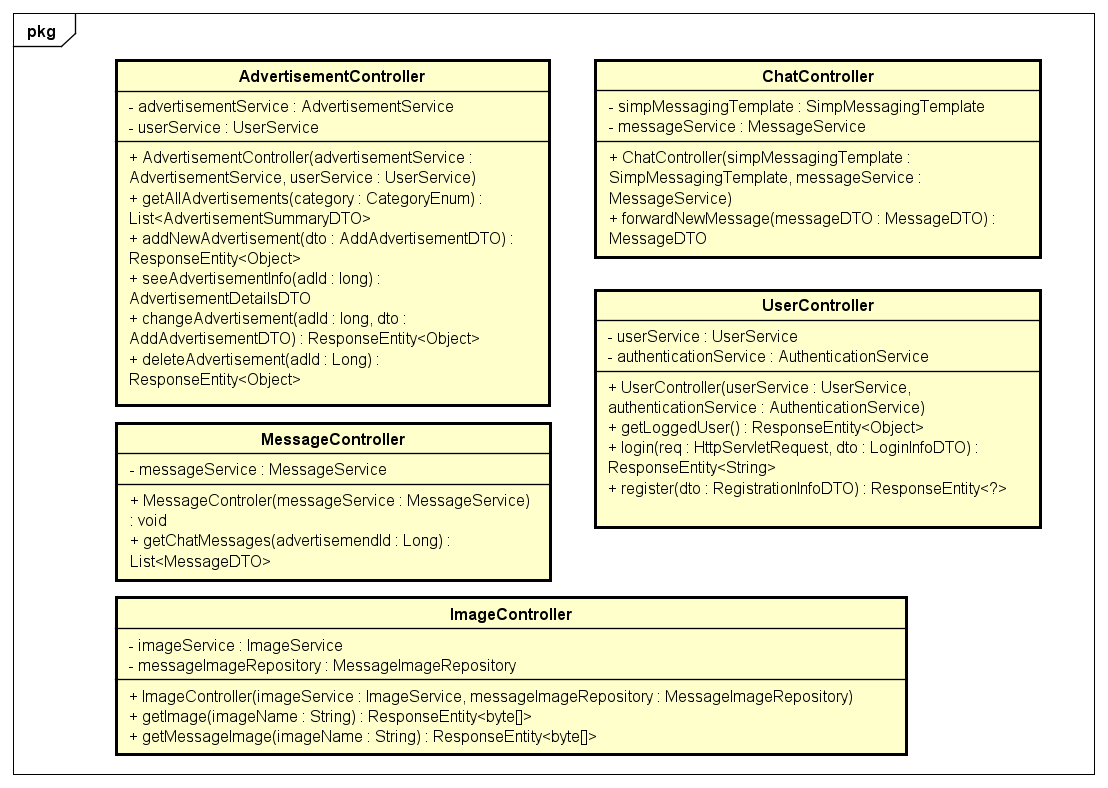
\includegraphics[width=\textwidth]{slike/controllersUML.png}
				\caption{Dijagram razreda - paket "controller"}
			\end{figure}
			\pagebreak

                Servisni sloj pruža poslovnu logiku i pristup podacima za različite funkcionalnosti aplikacije. Razredi paketa \textit{services} koriste repozitorije za pristup podacima. Rezultati ovih servisa se koriste u razredima koji se nalaze u paketu \textit{controller} kako bi se generirali odgovori na zahtjeve korisnika.
   
			\begin{figure}[htb]
				\centering
				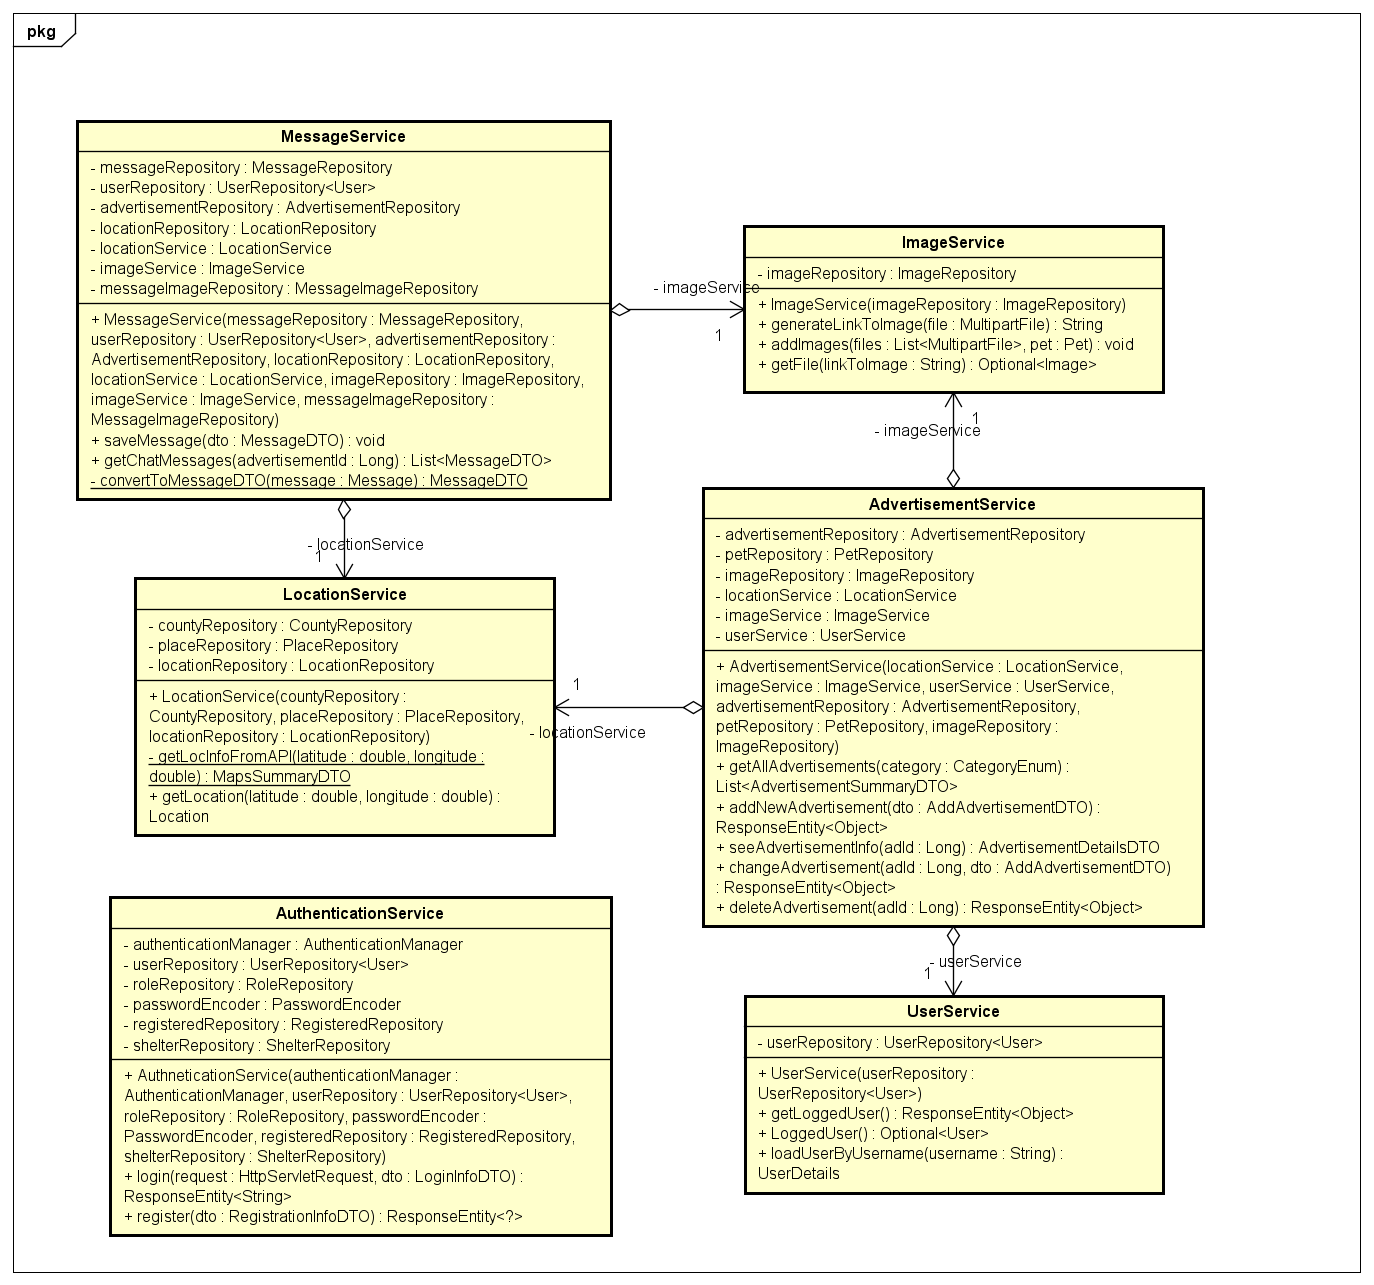
\includegraphics[width=\textwidth]{slike/serviceUML.png}
				\caption{Dijagram razreda - paket "services"}
			\end{figure}
			\pagebreak

                \textit{Entity} razredi odražavaju strukturu baze podataka u aplikaciji. Metode unutar ovih razreda komuniciraju izravno s bazom podataka kako bi dohvatili željene podatke. Razred \textit{User} predstavlja neregistriranog korisnika koji se može registrirati popunjavajući obrazac svojim osnovnim informacijama. Registrirane korisnike dijelimo na razred \textit{Registered} koji predstavlja korisnika koji je registriran i može koristiti osnovne funkcionalnosti sustava te na razred \textit{Shelter} koji predstavlja sklonište za životinje. Sklonište ima mogućnost oglašavanja pronađenih životinja.
   
			\begin{figure}[htb]
				\centering
				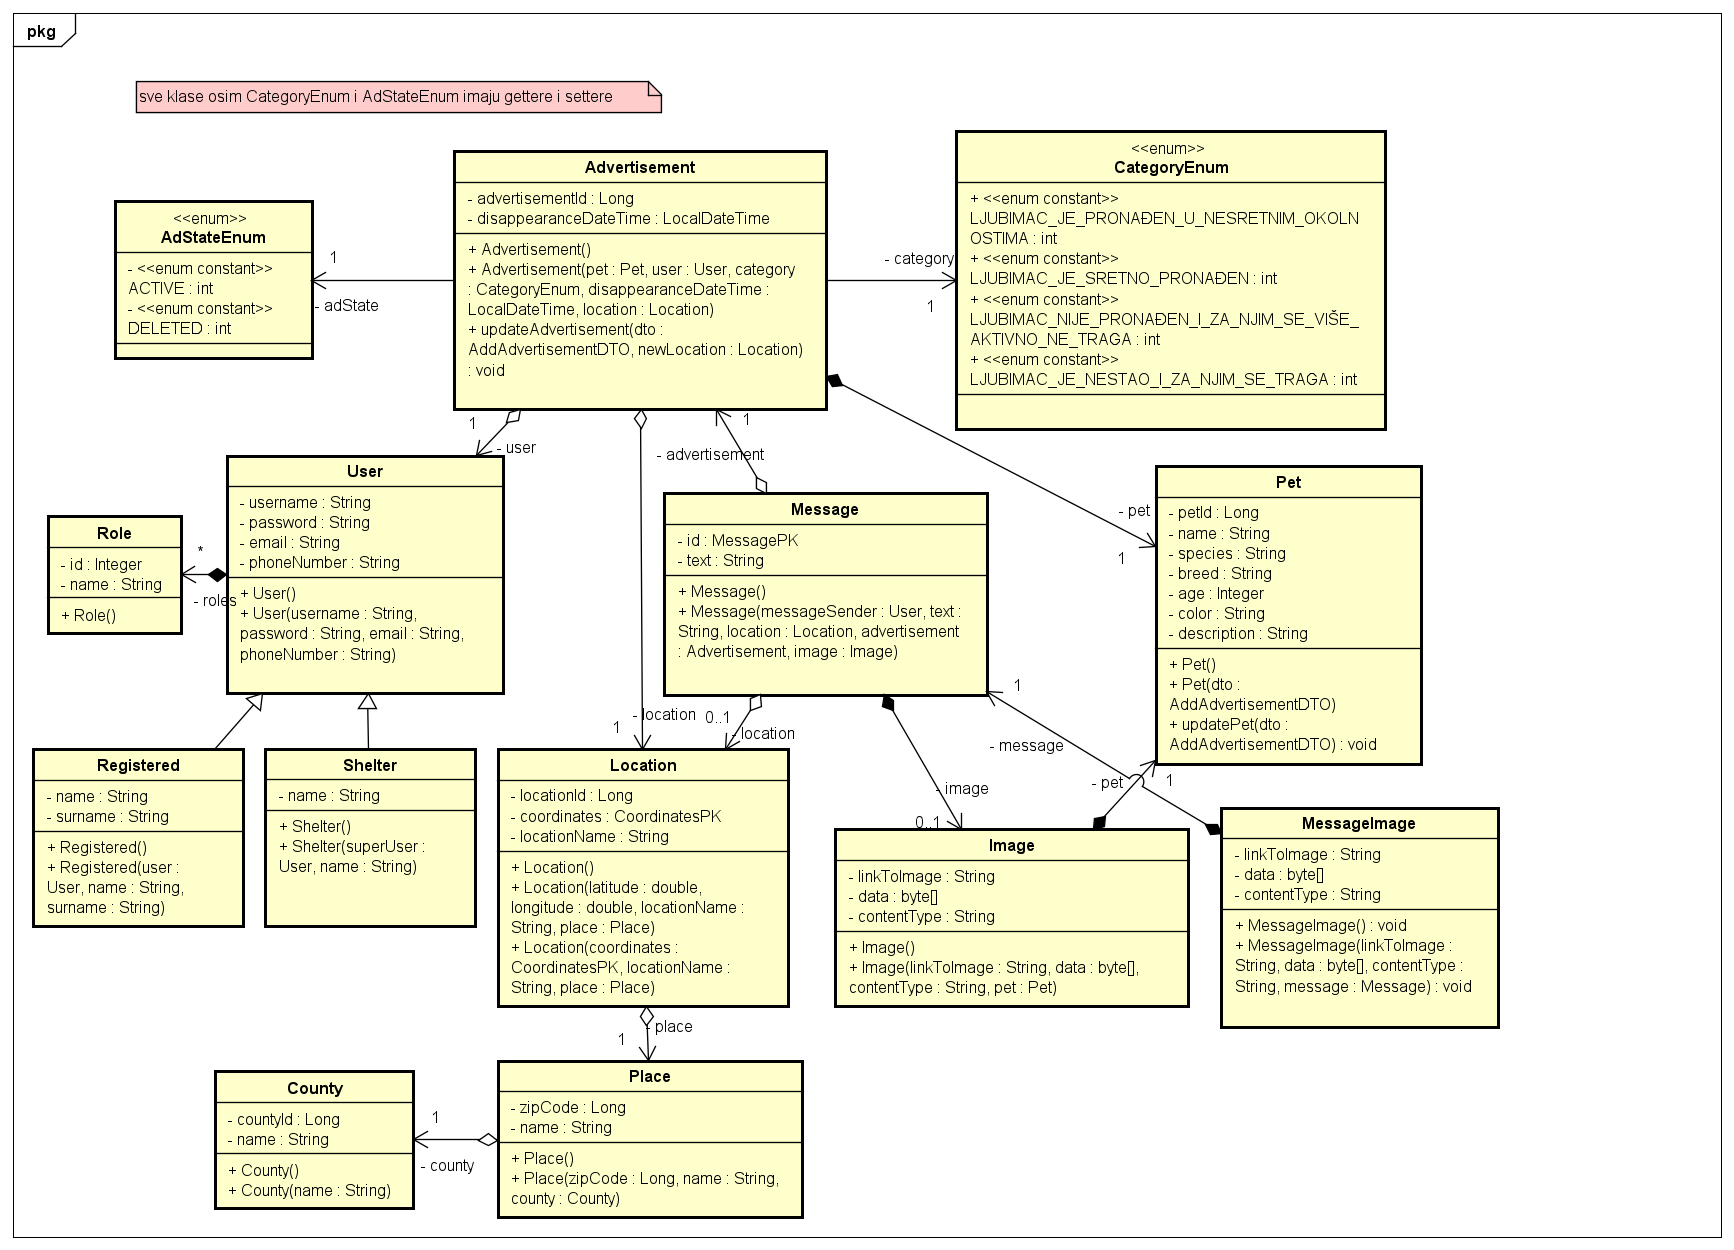
\includegraphics[width=\textwidth]{slike/entitiesUML.png}
				\caption{Dijagram razreda - paket "entity"}
			\end{figure}
			\pagebreak
			
			\begin{figure}[htb]
				\centering
				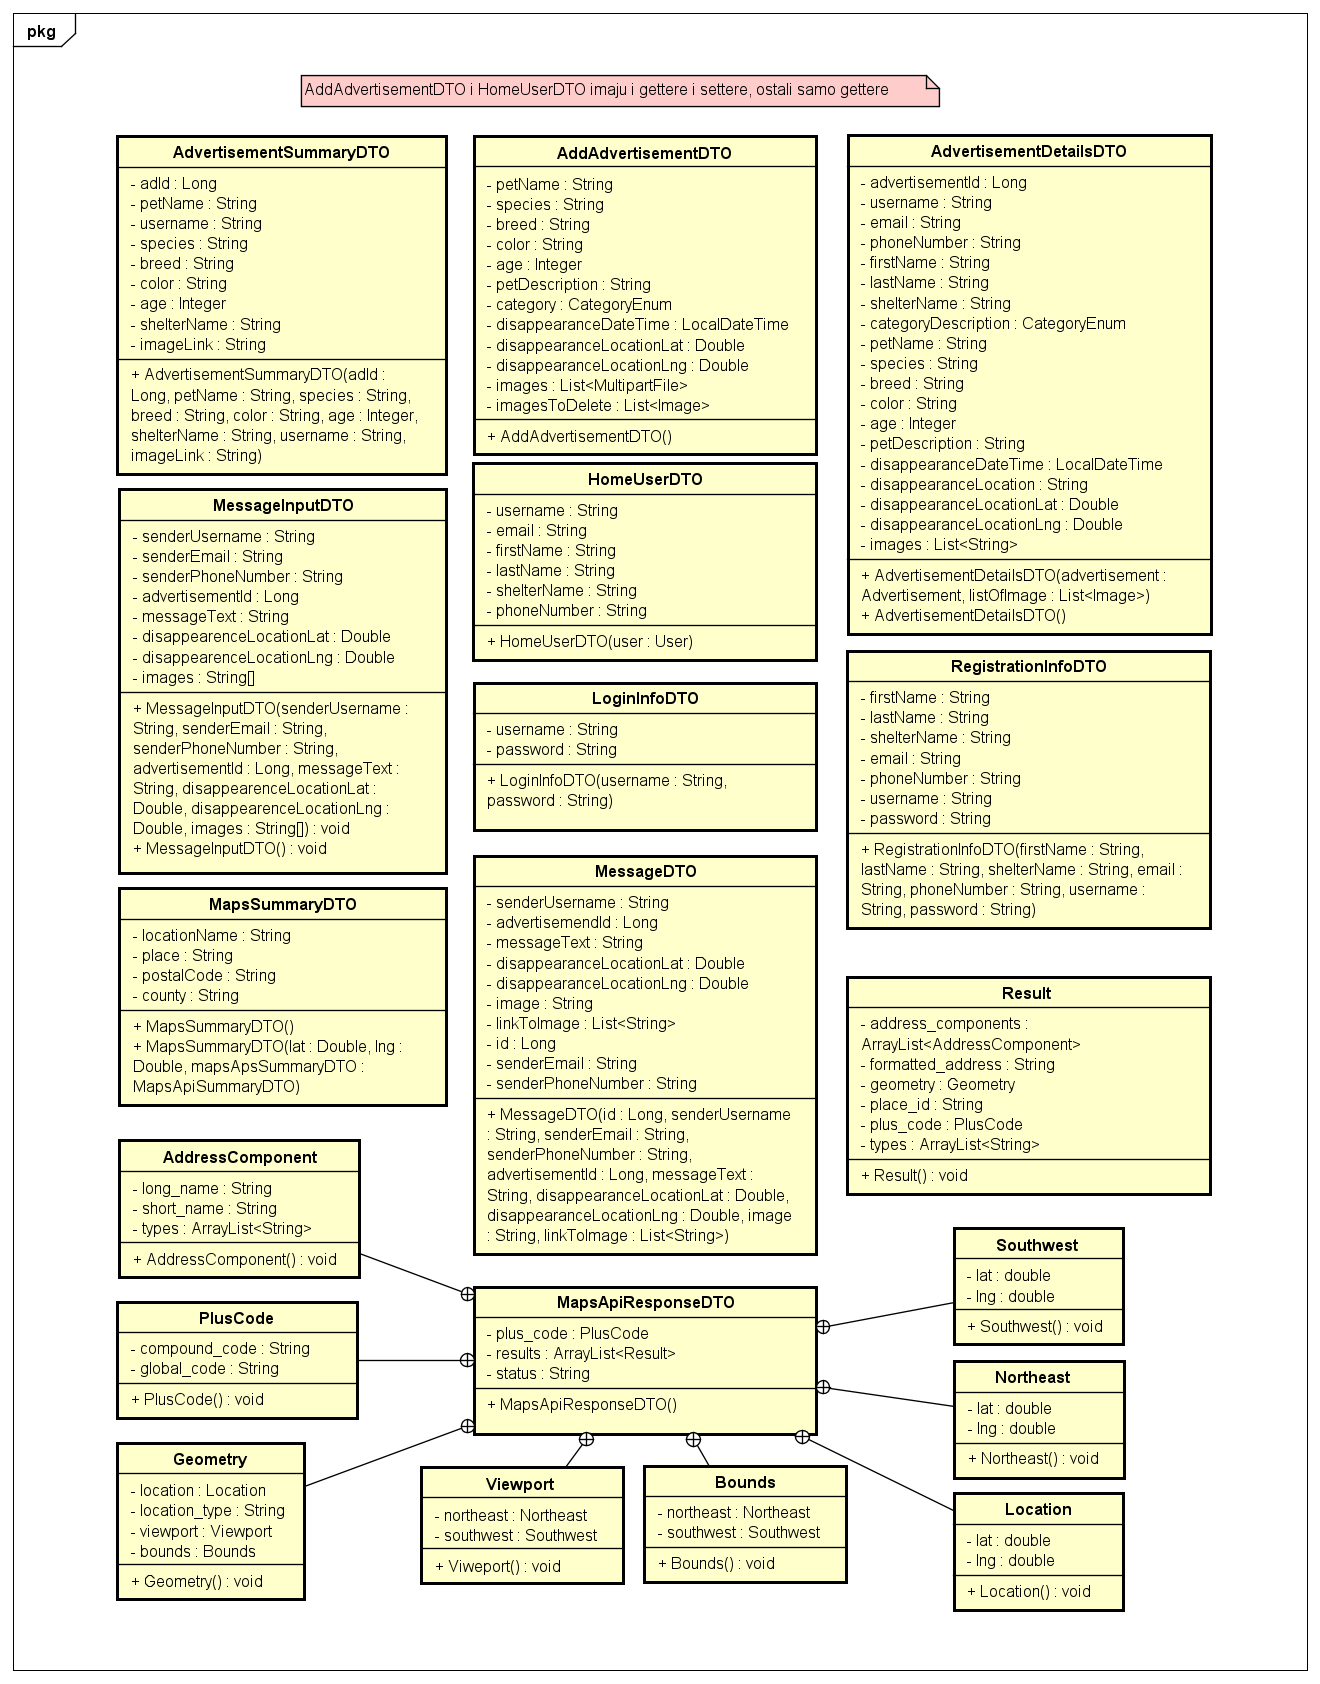
\includegraphics[width=\textwidth]{slike/dtoUML.png}
				\caption{Dijagram razreda - paket "dto"}
			\end{figure}
			\pagebreak

            \clearpage
            \newpage
            \eject
			
		\section{Dijagram stanja}
			
			
			\noindent Dijagram stanja prikazuje stanja objekta te prijelaze iz jednog stanja u drugo temeljene na događajima. Na slici 4.8 prikazan je dijagram stanja za registriranog korisnika. Nakon prijave, klijentu se prikazuje početna stranica na kojoj može pregledavati oglase. Za odabrani oglas, registrirani korisnik nadalje može pregledavati i sudjelovati u komunikaciji vezanoj uz potrazi za ljubimcem iz oglasa. S početne stranice klijent također može doći do opcija dodavanja oglasa te, u slučaju da je klijent objavio oglas, izmjene i brisanja oglasa.
			
			\begin{figure}[htb]
				\centering
				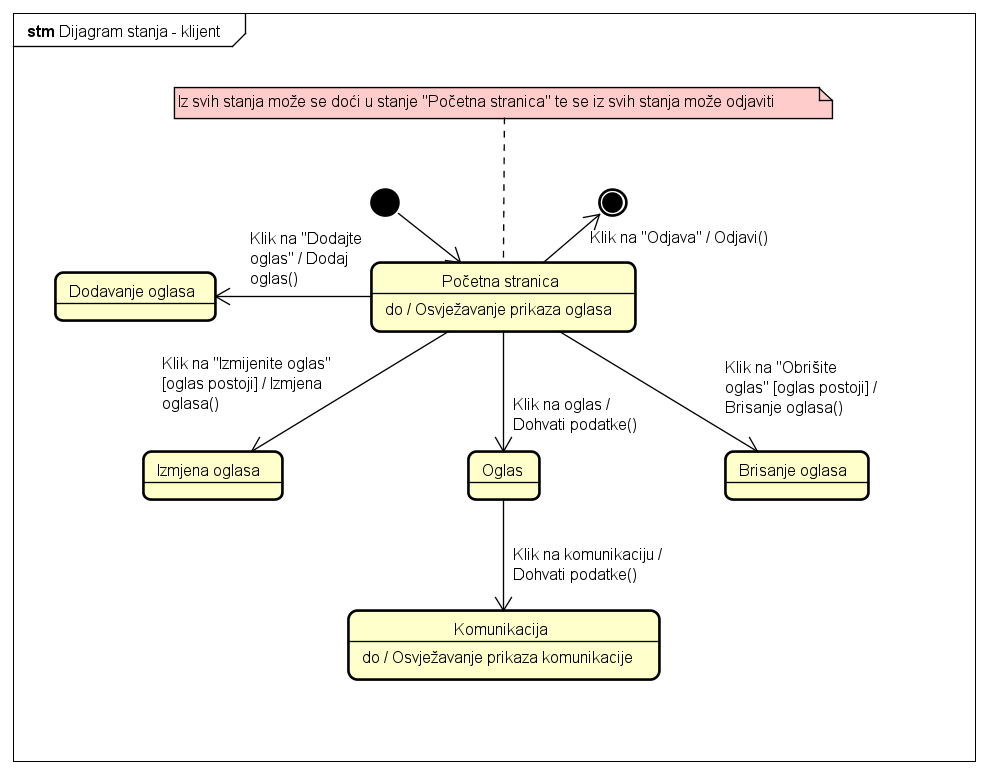
\includegraphics[width=\textwidth]{slike/Dijagram_stanja_-_klijent.png}
				\caption{Dijagram stanja - klijent}
			\end{figure}
			
			\eject 
		
		\section{Dijagram aktivnosti}
			
			\noindent Dijagram aktivnosti prikazuje izvođenje aktivnosti kroz niz akcija koje čine upravljačke tokove i tokove objekata. Na slici 4.9 prikazan je dijagram aktivnosti za slanje jedne poruke u potrazi za ljubimcem. Korisnik se najprije prijavljuje u web-aplikaciju, a zatim pretražuje oglase prema kategoriji po odabiru. Nakon pronalaska oglasa, registrirani korisnik može odabrati opciju za prikaz komunikacije vezane uz pronalazak ljubimca iz oglasa. Konačno, korisnik može poslati poruku koja se sprema u bazu podataka.
			
			\begin{figure}[!htb]
				\centering
				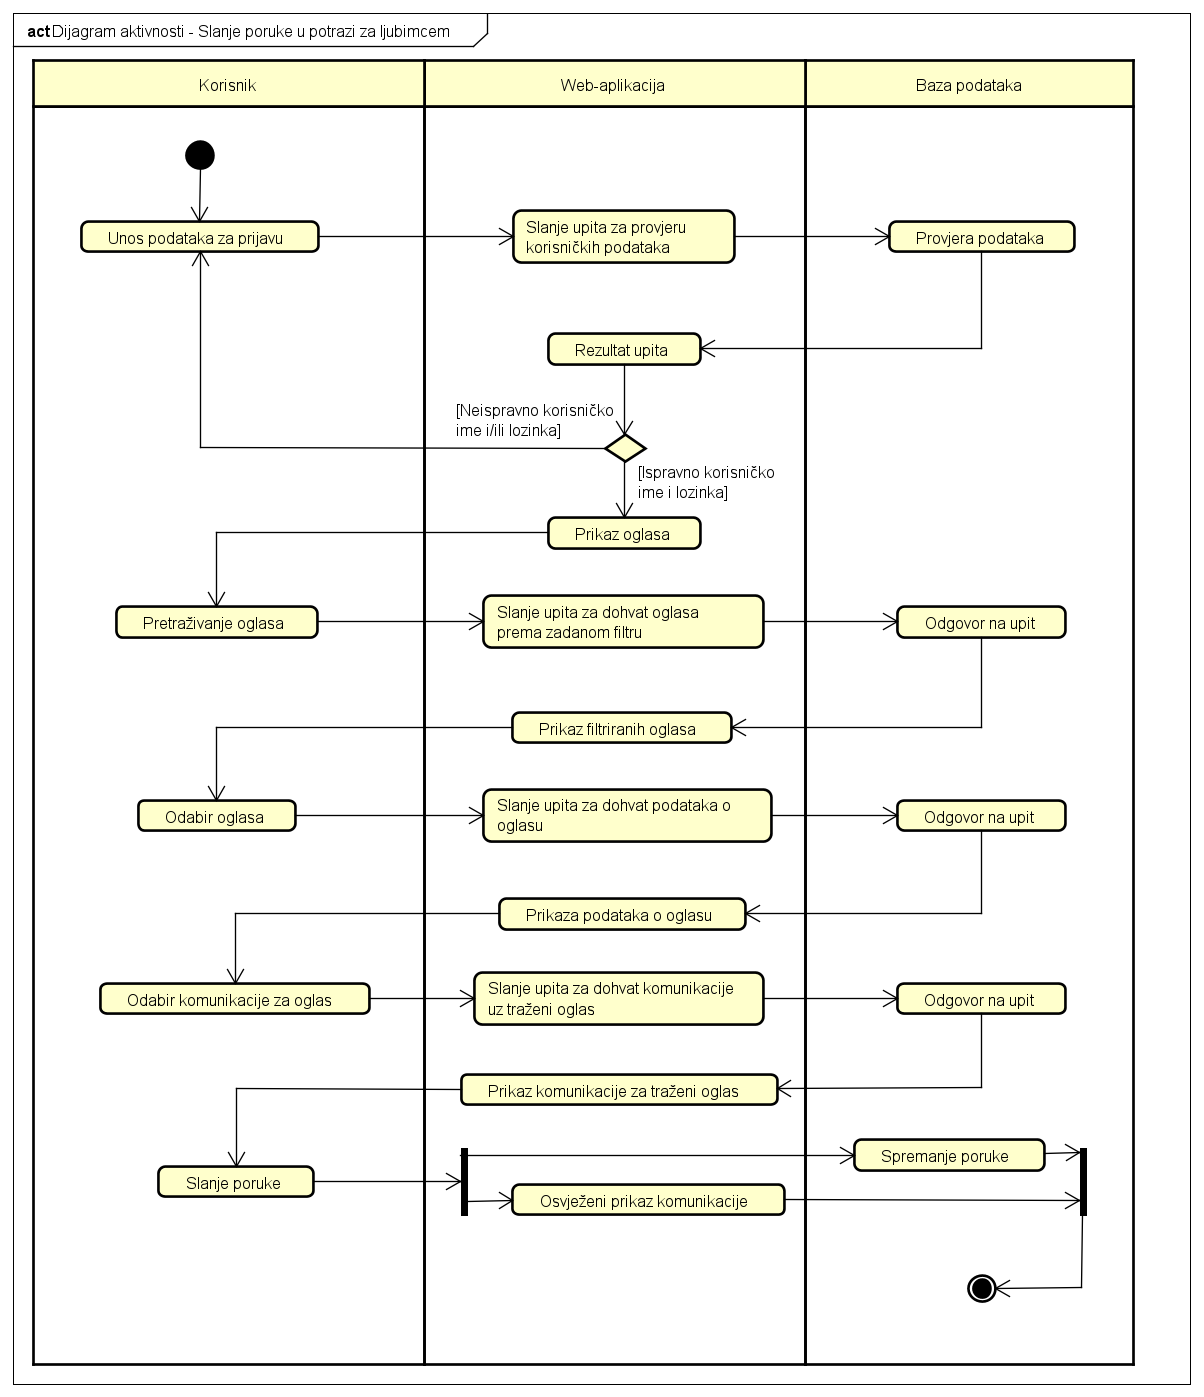
\includegraphics[width=\textwidth]{slike/Dijagram_aktivnosti_-_Slanje_poruke_u_potrazi_za_ljubimcem.png}
				\caption{Dijagram aktivnosti - Slanje poruke u potrazi za ljubimcem}
			\end{figure}

                \clearpage
                \newpage
                \eject
   
		\section{Dijagram komponenti}
		
			\noindent Dijagram komponenti, kao što je prikazano na slici 4.10, opisuje organizaciju, međuovisnost komponenti, te interne strukture i odnose prema okolini u sustavu. Sustav ima dva različita sučelja: sučelje za dohvat HTML, CSS i JS datoteka koje poslužuje \textit{frontend} dio aplikacije te sučelje za dohvat JSON podataka koje pristupa REST API komponenti. \textit{Frontend} dio sastoji se od niza JavaScript datoteka koje su grupirane u logičke cjeline prema tipovima aktora koji pristupaju aplikaciji. Sve JavaScript datoteke ovise o React biblioteci iz koje dohvaćaju gotove komponente kao što su gumbi, forme i slično. REST API poslužuje podatke koji pripadaju \textit{backend} dijelu aplikacije. Podaci se dohvaćaju putem REST API sučelja, a \textit{entity} je zadužen za dohvaćanje tablica iz baze podataka pomoću SQL upita. \textit{Backend} koristi MVC arhitekturu za slanje podataka u obliku dto \textit{(Data Transfer Object)} prema Reactview komponenti. React-view komponenta komunicira sa \textit{Nestali ljubimci} aplikacijom preko dostupnih sučelja. Ovisno o korisnikovim akcijama, osvježava prikaz, dohvaća nove podatke ili datoteke te ih prikazuje korisniku.

                \begin{figure}[!htb]
		      \centering
		    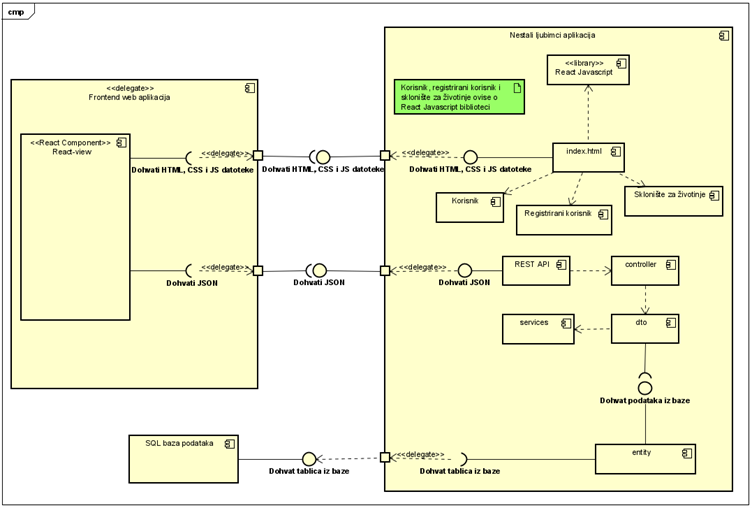
\includegraphics[width=\textwidth]{slike/Dijagram_komponenti}
		      \caption{Dijagram komponenti}
		      \end{figure}